\documentclass{article}
\usepackage[OT1]{fontenc} % Match official pdfLaTeX Times encoding under XeTeX as well.
\usepackage{microtype}
\usepackage{graphicx}
\usepackage{booktabs}
\usepackage{amsmath,amssymb}
\usepackage{array}
\usepackage{xurl}
\usepackage[hypertexnames=false]{hyperref}
\usepackage{mlsys2025}
\hypersetup{pdfauthor={Anonymous Authors},pdftitle={Predicting Native Intervention Outcomes in Speculative Decoding},pdfsubject={MLSys 2027 research manuscript v0.10.0},pdfkeywords={speculative decoding, correctness, runtime characterization}}
\newif\ifruntime
\ifdefined\HardwareOnly\runtimefalse\else\runtimetrue\fi
\newcommand{\microv}{V_k^{\mathrm{micro}}}
\newcommand{\vTwo}{V_2^{\mathrm{micro}}}
\newcommand{\dreal}{D_{\mathrm{real}}}
\newcommand{\rtarget}{R_{\mathrm{target}}}
% Generated from repository evidence by scripts/build_assets.py.
\newcommand{\MRepSpeed}{0.842}
\newcommand{\MRepN}{24}
\newcommand{\MRepPairs}{72}
\newcommand{\MRepExact}{72}
\newcommand{\MRepFaster}{1}
\newcommand{\MRepLo}{0.809}
\newcommand{\MRepHi}{0.877}
\newcommand{\MHEspeed}{1.387}
\newcommand{\MHEprompts}{30}
\newcommand{\MHEpairs}{90}
\newcommand{\MHEexact}{90}
\newcommand{\MHEfaster}{30}
\newcommand{\MHElo}{1.351}
\newcommand{\MHEhi}{1.422}
\newcommand{\MHEenergy}{1.013}
\newcommand{\MHEenergyLo}{0.990}
\newcommand{\MHEenergyHi}{1.034}
\newcommand{\RTXcpuSpeed}{0.404}
\newcommand{\RTXcpuLo}{0.390}
\newcommand{\RTXcpuHi}{0.418}
\newcommand{\RTXgpuSpeed}{0.650}
\newcommand{\RTXgpuLo}{0.629}
\newcommand{\RTXgpuHi}{0.673}
\newcommand{\RTXexact}{90}
\newcommand{\BSpeed}{0.3087}
\newcommand{\BLo}{0.2927}
\newcommand{\BHi}{0.3246}
\newcommand{\BvShort}{1.983}
\newcommand{\BvLong}{1.992}
\newcommand{\BExact}{60}
\newcommand{\BExactPrompts}{20}
\newcommand{\BFastExact}{45}
\newcommand{\RTXrawZero}{1.009}
\newcommand{\RTXserZero}{2.431}
\newcommand{\RTXrawDepth}{0.983}
\newcommand{\RTXserDepth}{2.137}
\newcommand{\HExact}{90}
\newcommand{\HcpuSpeed}{0.734}
\newcommand{\HcpuLo}{0.693}
\newcommand{\HcpuHi}{0.771}
\newcommand{\HcpuC}{2.4631}
\newcommand{\HcpuDraft}{12.63}
\newcommand{\HcpuTarget}{87.34}
\newcommand{\HcpuResidual}{0.04}
\newcommand{\HcpuD}{0.4304}
\newcommand{\HcpuR}{2.9767}
\newcommand{\HcpuX}{0.00124}
\newcommand{\HcpuAggregate}{0.7227}
\newcommand{\HnpuSpeed}{0.352}
\newcommand{\HnpuLo}{0.333}
\newcommand{\HnpuHi}{0.369}
\newcommand{\HnpuC}{2.4584}
\newcommand{\HnpuDraft}{58.35}
\newcommand{\HnpuTarget}{41.63}
\newcommand{\HnpuResidual}{0.02}
\newcommand{\HnpuD}{4.1251}
\newcommand{\HnpuR}{2.9435}
\newcommand{\HnpuX}{0.00130}
\newcommand{\HnpuAggregate}{0.3477}

% Generated from frozen runtime evidence by runtime_values.py.
\newcommand{\RTGuard}{1.3114}
\newcommand{\RTGuardLo}{1.2487}
\newcommand{\RTGuardHi}{1.3787}
\newcommand{\RTAlways}{1.3469}
\newcommand{\RTAlwaysLo}{1.2867}
\newcommand{\RTAlwaysHi}{1.4088}
\newcommand{\RTOracle}{1.0278}
\newcommand{\RTOracleLo}{1.0137}
\newcommand{\RTOracleHi}{1.0446}
\newcommand{\RTFallback}{30.6}
\newcommand{\RTK}{2}
\newcommand{\RTCap}{128}
\newcommand{\RTRounds}{8}
\newcommand{\RTMargin}{0}
\newcommand{\RTCalibration}{40}
\newcommand{\RTQualification}{16}
\newcommand{\RTPrompts}{60}
\newcommand{\RTQualPairs}{48}
\newcommand{\RTReps}{3}
\newcommand{\RTObservations}{540}
\newcommand{\RTExact}{180}
\newcommand{\RTBootstrap}{10,000}
\newcommand{\RTSeed}{20260924}
\newcommand{\RTSecondary}{1.0271}
\newcommand{\RTSecondaryLo}{1.0130}
\newcommand{\RTSecondaryHi}{1.0436}
\newcommand{\RTGuardFaster}{24}
\newcommand{\RTAlwaysFaster}{36}
\newcommand{\RTTies}{0}

% Generated by scripts/direct_id_values.py from frozen formal JSON; do not edit.
\newcommand{\DIRTXBatchedPairs}{75}
\newcommand{\DIRTXBatchedPrompts}{25}
\newcommand{\DIRTXBatchedStatus}{BLOCKED}
\newcommand{\DIRTXSerializedPairs}{90}
\newcommand{\DIRTXSerializedPrompts}{30}
\newcommand{\DIRTXSerializedStatus}{QUALIFIED}
\newcommand{\DIBFastPairs}{60}
\newcommand{\DIBFastPrompts}{20}
\newcommand{\DIBFastStatus}{BLOCKED}
\newcommand{\DIBSerializedPairs}{78}
\newcommand{\DIBSerializedPrompts}{26}
\newcommand{\DIBSerializedStatus}{BLOCKED}

% New campaign projection; historical macros remain unchanged.
\newcommand{\FUCost}{0.646}
\newcommand{\FUCostLo}{0.630}
\newcommand{\FUCostHi}{0.660}
\newcommand{\FUForkScores}{72}
\newcommand{\FUForkImmediate}{0}
\newcommand{\FUForkLater}{18}
\newcommand{\FUForkLaterPrompts}{6}
\newcommand{\FUForkEvents}{195}

% Post-study existing-record derived values; no original primary macro altered.
\newcommand{\DerCPUZero}{0.8275}
\newcommand{\DerNPUZero}{0.8352}
\newcommand{\DerAlwaysOracle}{1.0007}
\newcommand{\DerTargetFaster}{2}
\newcommand{\DerScoreAbsMedian}{0.0695}
\newcommand{\DerScoreAbsMax}{2.3503}
\newcommand{\DerMarginMin}{0.2291}
\newcommand{\DerMarginAltMin}{0.2003}
\newcommand{\DerRTXTargetMs}{1907.9}
\newcommand{\DerRTXSerialMs}{2923.3}

% RTX V4 primary estimates; original campaigns and macros are unchanged.
\newcommand{\VFourCost}{0.677}
\newcommand{\VFourCostLo}{0.662}
\newcommand{\VFourCostHi}{0.692}

% Post-study retained-record diagnostics; historical macros unchanged.
\newcommand{\DiagBNonref}{155}
\newcommand{\DiagBAfter}{151}
\newcommand{\DiagCPUCeiling}{0.8372}
\newcommand{\DiagNPUCeiling}{0.8448}
\newcommand{\DiagCPUReduction}{16.28}
\newcommand{\DiagNPUReduction}{15.52}
\newcommand{\DiagMOpportunity}{0.069}

\mlsystitlerunning{Predicting Native Intervention Outcomes}
\begin{document}
\twocolumn[{
\mlsystitle{Predicting Native Intervention Outcomes in Speculative Decoding}
\begin{mlsysauthorlist}
\mlsysauthor{Anonymous Authors}{anon}
\end{mlsysauthorlist}
\mlsysaffiliation{anon}{Anonymous Institution}
\mlsyscorrespondingauthor{Anonymous Author}{anon.email@domain.com}
\mlsyskeywords{speculative decoding, correctness, runtime characterization}
\vskip 0.3in
\begin{abstract}
A reference mismatch rejects an execution path but does not describe its later output or predict a controlled intervention. We test frozen executable execution-path descriptions against complete native generated-ID arrays and endpoints before and after stage-specific changes. On one B570 stack, draft-free predictions match both conditions on 24 exposed tasks, and a prefill intervention restores all four diagnostic deviations without new control deviations. On one RTX stack, proposal-conditioned predictions match both conditions on 43 tasks, yet a target-continuation intervention fails its reference-recovery and no-new-regression goal: one task recovers and one newly deviates, leaving aggregate agreement unchanged. These distinct finite tests establish intervention-prediction closure, not universal repair, functional correctness or a unique stage cause. Separate cost evidence finds qualified RTX serialization slower, conditional 358H overhead-removal ceilings below parity, and M4 Guard inferior to fixed speculation. Complete prediction, paired reference effects and realized cost support different system decisions.
\end{abstract}
}]
\printAffiliationsAndNotice{}
\ifruntime\else
\hypersetup{pdfsubject={MLSys 2027 v0.10.0 internal hardware-only proof}}
\noindent\textbf{Internal section-removal and reference proof only.}
\fi
\section{Introduction}
\label{sec:intro}
Speculative decoding promises lower serial decoding latency by using a cheaper draft model to propose tokens that a target model validates together \citep{leviathan2023}. High acceptance, fast drafting, and cheap batched target execution can each make an implementation look promising. We ask what prevents those local indicators from translating into gains in integrated post-prefill speculative decode on the tested consumer configurations, and whether the measured constraints can guide runtime decisions.

We investigate MacBook Air M4, Core Ultra 9 275HX with RTX 5070 Ti Laptop, Core i5-13400 with Arc B570, and Core Ultra X7 358H with Arc B390 and CPU/NPU drafting. Outcomes differ sharply even within a platform. The representative M4 workload is token-exact but reaches only \MRepSpeed$\times$ speedup; a separately preregistered HumanEval workload on the same M4 is exact and reaches \MHEspeed$\times$. Differing session conditions prevent attributing this contrast to workload alone. Profitability is not a simple hardware capability in these studies.

Two diagnoses explain important failures elsewhere. On RTX 5070 Ti Laptop, correctness qualification removes cheap batching; the tested exact serialized controls cost more. B570 serialization improves agreement without qualifying the full workload. On 358H, the isolated NPU draft advantage does not survive the tested stateful integration, while complete target-side work dominates CPU drafting. These diagnoses neither exhaust possible causes nor explain the M4 contrast. Hardware, workload, and runtime co-vary; all gains concern post-prefill decode, excluding loading and initial prompt prefill.

Our contribution combines retrospective consumer-stack characterization with separately frozen runtime studies. The characterization retains positive, negative, and correctness-blocked outcomes, using path controls and direct timing to distinguish component promise from realized cost. Runtime qualification then blocks the tested 358H intervention before formal performance evaluation. On an exact M4 path, a guard using already-realized cost achieves profitable held-out execution against target-only, although fixed speculation has a higher aggregate point estimate. The studies connect correctness-qualified paths to measured control decisions. Performance characterization, heterogeneous placement, cost/commit accounting, and deterministic speculation have prior art \citep{dovetail,duodecoding,illusion,specllm,llm42}; our contribution is this bounded empirical connection, not a new speculative algorithm or universal profitability theory.

\section{Questions, Output Contract and Cost}
\label{sec:framework}
We distinguish three questions: can an execution description predict a trajectory, does that trajectory preserve a specified reference, and does a qualified implementation reduce complete cost? Acceptance rate, isolated draft throughput and target-forward batching answer narrower questions.

\subsection{Prediction and reference compatibility}
Let $k$ be maximum draft width, UB the target micro-batch capacity ($n_{\mathrm{ubatch}}$), and EOG a vocabulary end-of-generation ID. A greedy speculative round verifies proposals, commits the agreeing prefix and a correction or bonus when budget permits, then removes inconsistent suffix state. Our strict output contract compares complete committed generated IDs with the matched target-only greedy reference under the frozen model/runtime/configuration. A failed pair blocks a workload-global lossless optimization claim; a small passing probe establishes eligibility for a larger gate. Capped ID equality does not measure functional HumanEval correctness or pass@$k$.

Historical text-path agreement (H) compares arrays reconstructed from CLI text. Direct-ID qualification (Q) compares captured IDs with the study's reference. Prediction equality compares a sealed complete array with reserved native live IDs. Prediction can succeed on a reference-divergent path, so it does not imply Q. We write prediction equality in words; the letter P below denotes only the draft worker. Same-state intervention has separate score, immediate-decision and continuation endpoints.

\subsection{Execution descriptions as testable candidates}
Table~\ref{tab:inputcontracts} states what each program receives and computes. UB denotes capacity, not a trace of actual forward shapes, occupied positions or prior KV operations. In particular, target-only UB2 and native speculative UB2 need not issue the same sequence of forwards. The candidate test checks complete output directly. Equal parameter names alone do not establish equal numerical paths.
\begin{table*}[t]
\caption{Inputs and local execution contracts. Each program starts from its own prompt prefill. P = draft worker; R = target worker. Shared numerical routines limit implementation independence. UB labels do not specify identical actual forward traces.}
\label{tab:inputcontracts}
\centering
\begin{tabular}{@{}>{\raggedright\arraybackslash}p{1.03in}>{\raggedright\arraybackslash}p{1.43in}>{\raggedright\arraybackslash}p{2.00in}>{\raggedright\arraybackslash}p{1.54in}@{}}
\toprule
Program & Generation inputs & Locally computed history / decisions & Separation or missing equivalence \\
\midrule
B570 H1 & Prompt; target weights; UB1; no draft or proposals & Own target-only generated prefix, KV and greedy decisions & Draft-free predictor; no unique-cause isolation \\
RTX target-only UB2 & Prompt; target weights; UB2; no draft or proposals & Own target-only prefix and KV; one generated-ID stream & Capacity-level candidate; equality of actual native forward traces is not established \\
RTX H2 & Prompt; P's proposals from its own earlier R feedback & R checks own prefix/pending ID; computes sampling, accept/correct/bonus and KV rollback & Separate P/R orchestration; shared llama.cpp/GGML/CUDA \\
RTX fresh R\_ONLY & Prompt; sealed H2 proposal requests, read sequentially & Fresh R computes its own target decisions and state transitions & Target-only execution of tape; tape generation uses draft; same numerical routines \\
Native RTX live & Prompt; its own draft proposals; no tape import & Native target/draft history, acceptance and state transitions & Independent live outcome; not an independent numerical implementation \\
\bottomrule
\end{tabular}
\end{table*}


\subsection{Complete realized cost}
Let $T_b$ be matched target-only cost per output token, $T_d^{\mathrm{real}}$ complete realized draft-subsystem time including interface replay, $T_{\mathrm{target,round}}^{\mathrm{real}}$ complete target work, and $T_x$ residual synchronization, transfer and bookkeeping outside those regions. Let $C$ count all committed output per round, including correction/bonus. Then
\begin{align}
S &= \frac{T_b C}{T_d^{\mathrm{real}}+T_{\mathrm{target,round}}^{\mathrm{real}}+T_x}\label{eq:physical}\\
 &= \frac{C}{\dreal+\rtarget+X}.\label{eq:normalized}
\end{align}
The normalized denominator gives break-even $C>\dreal+\rtarget+X$. These are accounting identities, not new profitability theory \citep{specllm}. Total-time ratios need not equal prompt geometric means. Incompatible experiments cannot isolate an unmeasured component by subtraction. The historical target-forward proxy $\microv$ omits drafting and integration; its original cells and separate fresh qualification gates remain in Appendix F.

Primary results retain their frozen questions and gates; post-study results are identified separately. Timing on blocked paths remains diagnostic, and a later Q gate does not certify historical H timing.

\section{Study Design and Evidence Scope}
\label{sec:methods}
\subsection{Frozen systems and complete endpoints}
Each study has its own protocol, tasks and comparator, stated beside its results and mapped in the historical appendix and the separate intervention appendix. The target/draft pair is Qwen3-8B/0.6B Q8\_0, except the 358H adapter's symmetric INT4 OpenVINO draft. Final comparisons process one request at a time. Historical settings are in Appendix K and RTX V4 in Appendix Q; hardware, backend, OS and quantization jointly vary, preventing hardware-only causal comparisons. RTX's original direct-ID OS build is 26200; follow-ups use 26300. A driver version alone does not identify driver bytes.

``Complete'' retains each protocol's generated-ID and endpoint rules: prompt IDs and uncommitted proposals are excluded; an earlier terminal EOG is inclusive, otherwise the 128-ID cap applies. Agreement compares all IDs within that endpoint and the endpoint itself. B570 raw native captures additionally retain 1--2 committed post-cap IDs, excluded from agreement but exported for audit. Actual stop markers are checked. Valid results are selected from each result manifest's complete attempt; failed or interrupted attempts are retained separately and are never concatenated.

The B570 intervention uses a previously exposed 24-task diagnostic/control cohort. RTX uses the old 19-task cohort and a separately frozen 24-task MBPP cohort; its candidate, exposure exclusions and static task order precede new-task execution. Frozen prediction arrays precede native runs. RTX additionally records remote readback before native; B570 uses local seals. Neither provides independently trusted absolute experimental time. Prospective prediction is not equivalent to formal independent preregistration, and the candidate's earlier exposure is recorded. No tasks are added or dropped after observing these results. Three repeats assess within-task stability; finite exact counts receive no pseudo-independent binomial intervals.

The offline intervention review restores the hash-bound evidence archive and independently parses selected result/raw/trace records. It checks prediction/native and native/reference arrays and endpoints, repeat stability, paired transitions, handoff witnesses, shams, graph occupancy and effective settings. Opaque sampler state cannot be serialized: clone behavior and checked surrounding state do not establish byte equality of opaque sampler bytes. Omitted weights/runtime binaries remain identified but are not independently rehashed or executed by this review. The author evidence packet records exact review coverage and source/hash bindings.

Historical M4 includes a representative 24-prompt Spec-Bench sample \citep{specbench} and a separate preregistered 30-task HumanEval study \citep{humaneval}; they are background, not replications of the later runtime study. The latter retains its own calibration, qualification and held-out splits in \ifruntime Section~\ref{sec:runtime}\else the full manuscript\fi. All studies keep their original stop rules and comparators.

\subsection{Cost estimators and conditional uncertainty}
Later RTX cost studies take each condition's median of three times per prompt, then reference/candidate ratios and their prompt GM. V4 uses 10,000 paired-row bootstrap draws, seed 2026100204, frozen task order and linear .025/.975 percentiles. This resamples the empirical distribution of the selected prompt rows, conditional on the exposure-audited cohort, observed condition medians and frozen configuration. It does not account for exposure selection, predict a HumanEval population failure rate or cover a new thermal/session distribution. Repetitions are not independent bootstrap units. Cost interpretation requires every reference-ID pair and stable reference repeats; blocked timing remains diagnostic.

The 358H prompt estimator takes the median of three paired ratios before the prompt GM; total-time accounting is separate. M4 runtime uses condition medians and its own frozen random streams. Historical H estimators remain in Appendix B. All intervals omit full session and recalibration uncertainty.

Timing excludes loading and initial prefill. The RTX V4 timer begins after synchronized target/draft prefill and before per-request sampler/state work, ending at slot release. The M4 and 358H boundaries differ and are stated with their results. M4 package energy excludes separate DRAM, B570 uses adapter-board energy, and RTX mixed domains do not form a common system boundary. There is no end-to-end 358H Phase-3 or runtime energy result.

\subsection{Offline reproducibility}
The anonymous index recomputes retained arrays, timer intervals and summaries; the author packet supplies source/hash bindings and raw-review coverage. Appendix O maps historical entries and Q the V4 capabilities. Verification runs no models and does not authenticate omitted assets or absolute process time.

\paragraph{Existing-record analysis.}
Score/margin descriptors, trajectory extents, fixed-mode opportunity and conditional cost bounds are calculated after aggregate outcomes are known. Extent/budget analyses retain original rows and comparators without adding samples or intervals. V4 latency summaries describe 19 prompt medians per condition without changing the paired GM/CI. Appendix P gives the derivations.

\section{Prospective Execution-Path Prediction}
\label{sec:results}
\label{sec:diagnoses}
% B570 prediction summary from frozen discovery and reserved validation.
% This replaces the generic evaluation-flow graphic; no new result is inferred.
\begin{figure*}[t]
\centering
\small
\begin{tabular}{@{}p{0.95in}p{2.12in}p{3.08in}@{}}
\toprule
Stage & Design or comparator & Complete generated-ID endpoint \\
\midrule
Discovery & 12 prompts $\times$ 3 runs; select target-only UB1 as H1. & UB1 predicts the serialized trajectory in \textbf{36/36} runs. \\
Hypothesis freeze & After discovery; fix H1, reference, tasks and endpoint. & Before reserved reference/predictor inference; H2 remains unrun. \\
Prediction freeze & After pre-live inference; seal all 72 UB1 arrays. & Before the first reserved live outcome; no prediction edits. \\
Live test & Compare each of 72 live serialized runs with both frozen paths. & UB1 predictor/live \textbf{72/72}; UB128 reference/live \textbf{60/72 (BLOCKED)}. Four prompts (12 runs) are reference-divergent. \\
Divergent case & HumanEval/134; first difference at generated-ID index 88. & Reference ID 914 $\rightarrow$ predictor/live ID 1946 in all 3 runs. \\
\bottomrule
\end{tabular}
\caption{\textbf{B570 prospective prediction.} Hypothesis and full-array freezes are separate stages. The 24 prompts $\times$ three repeat-stable runs test complete capped trajectories, including four non-reference predictions. Reported ordering and retained arrays are reviewed in the appendix; prediction success does not restore qualification.}
\label{fig:translation}
\end{figure*}

\subsection{B570: a draft-free full-trajectory predictor}
\label{sec:b570mechanism}
A target-only harness first reproduces 90/90 UB128 reference sequences. On 12 exposed discovery tasks, H1 target-only UB1 matches 36/36 native serialized trajectories. The frozen decision tree selects H1 and leaves H2 unrun. Conservative exposure exclusion then selects 24 reserved tasks. H1 freezes before reserved reference/predictor inference, and all 72 complete predictions freeze before reserved native live (Figure~\ref{fig:translation}).

Prediction/live agrees 72/72 over three stable runs per prompt, including all 12 runs of four reference-divergent prompts. The same-set UB128 reference agrees only 60/72 and remains \emph{BLOCKED}. Every reserved array reaches 128 generated IDs. Any wrong later ID would falsify the prediction, rather than merely reproduce a first-difference signature. The four first differences occur on /134 at index88 (914$\to$1946), /42 at 73 (432$\to$1817), /145 at 103 (1184$\to$686), and /138 at 93 (14374$\to$9064); all later IDs are also predicted. Appendix J retains every committed array and freeze role.

This answers a question that qualification alone cannot. Reference mismatch establishes that the path is unsuitable for strict replacement; it does not establish whether a target-only program can describe its full output. Here the selected target-only UB1 program suffices without receiving draft weights, proposals or future live IDs. That result rules out the need for those inputs \emph{in this successful predictive description}. It does not show that drafting is causally irrelevant inside native execution, that UB1 is the unique predictor, or that the output contract is restored.

\subsection{Sampled numerical sensitivity is not an immediate split}
A separate frozen fork study uses 24 new prompts $\times$ three, sampling the first verification block after at least 64 committed IDs. UB1/UB128 branches share checked KV, prefix, positions, proposals and cloned sampler state. Scores change at \FUForkScores/72 forks, but raw top-one and actual immediate decisions change at \FUForkImmediate/72. The immediate comparison contains 195 reachable paired decisions; 216 raw-logit rows are correlated within prompts and blocks.

\begin{samepage}
Existing-record descriptors put these results on a score scale. Median absolute top-one score change is \DerScoreAbsMedian, with p95 0.3437 and maximum 2.3503. Raw top-two margins have minima 0.2291 (UB1) and 0.2003 (UB128), and medians 17.5021 and 17.5128. These are marginal descriptors, not a certified decision-boundary distance or a uniform perturbation bound. In particular, the study does not supply a sampled near-tie witness. Changed scores with stable sampled decisions show local numerical sensitivity and immediate stability, not a whole-generation null effect.
\end{samepage}

The alternate branch restores draft state and continues with UB128 target blocks; later proposals follow its altered live history. Complete trajectories differ in \FUForkLater/72 runs on \FUForkLaterPrompts/24 prompts, first diverging 10--50 positions after the fork. Persistent continuation therefore confounds attributing a delayed difference to one sampled block. The study neither explains the original H1 four tasks nor establishes immediate reference restoration. Appendices L/P retain score/margin distributions, all six later-sensitive prompts and clone/R0 controls.

\subsection{RTX: discriminating predefined candidates on one set}
\label{sec:rtxreplay}
Earlier RTX H1 fails exposed discovery at 24/36 and stops with zero reserved runs. A separate V2 study obtains 72/72 matches from proposal-conditioned H2 and fresh R\_ONLY but lacks a same-set target-only competitor (Appendix M). V4 addresses that missing comparison; it is not a retest of one portable B570 predictor.

All 19 remaining exposure-audited tasks enter V4. Four pre-live conditions---UB1 reference, target-only UB2, H2 and fresh R\_ONLY---produce 228 complete arrays. All arrays/tapes are sealed and remotely retrieved before 57 native batched live runs. H2's draft worker P uses its own earlier target feedback to construct proposals; target worker R computes its own decisions. Fresh R\_ONLY reads the sealed tape sequentially, and native live imports no tape. This separates application/API orchestration on shared llama.cpp/GGML/CUDA numerical routines (Table~\ref{tab:inputcontracts}), not adversarial OS access or an independent numerical implementation.

Table~\ref{tab:rtxv4trajectory} shows complete-array agreement and the cross comparison hidden by aggregate totals. Target-only UB2/live is 51/57 on 17/19 prompts. H2/live, R\_ONLY/live and H2/R\_ONLY are each 57/57; both programs predict the two reference-divergent trajectories. All five conditions are repeat-stable. UB2 and reference both score 51/57, but /18 refutes only the reference and /25 only UB2; /15 refutes both.
\begin{table}[t]
\caption{RTX V4 complete prediction/live agreement on 19 prompts $\times$ three. Separate P/R orchestration uses shared numerical routines. Below: full-array failures on all distinguishing tasks, stable in three repeats; replay matches every task. These are prediction comparisons, not qualification.}
\label{tab:rtxv4trajectory}
\centering
\begin{tabular}{@{}lrr@{}}
\toprule
Predictor / comparator & Pairs / 57 & Prompts / 19 \\
\midrule
Target-only UB2 & 51 & 17 \\
Separate P/R (H2) & 57 & 19 \\
Fresh R\_ONLY & 57 & 19 \\
UB1 reference & 51 & 17 \\
\bottomrule
\end{tabular}
\par\smallskip
\begin{tabular}{@{}llll@{}}
\toprule
Task & UB2 & Reference & H2 / R\_ONLY \\
\midrule
/15 & Fail & Fail & Match / Match \\
/18 & Match & Fail & Match / Match \\
/25 & Fail & Match & Match / Match \\
Other 16 & Match & Match & Match / Match \\
\bottomrule
\end{tabular}
\end{table}


The prospective result rejects the specified UB2 program's full-cohort sufficiency. Matching capacity does not establish identical occupied forward shapes, inputs or prior state transitions. Replay supplies a successful richer execution description; its success does not reject every target-only hypothesis or prove proposal/history necessary, minimal or unique. Tape construction uses drafting, and replay shares numerical code. Appendix Q gives first-difference IDs, complete endpoints and the failed V3 capture history; V3 contributes no observations to these denominators.

\section{From Local Opportunity to Realized Gain}
\label{sec:diagnoses}
We test output qualification, frozen path prediction and sampled intervention effects, then examine realized cost on a qualified path. Figure~\ref{fig:translation} shows the original B570 discovery, freeze and reserved test; later studies use their own tasks and gates.

\subsection{Execution-path qualification}
\label{sec:admissibility}
Figure~\ref{fig:verification}A retains eleven historical target-forward proxy cells. Metal $\vTwo\approx1.02$--$1.08$, near-step RTX batching, and B570 fast 1.24--1.64 versus serialized \BvShort--\BvLong\ describe different runs and contexts. Lower proxy values mean cheaper target-forward work relative to one-token decode. These measurements omit integration, cannot replace complete $\rtarget$, and have no same-study matched cost/qualification tradeoff with Panel B.

Original RTX and B570 direct-ID campaigns each use 30 prompts $\times$ three, with no timing and a 90/90 gate. RTX matches \DIRTXBatchedPairs/90 batched and \DIRTXSerializedPairs/90 serialized; only serialization qualifies. B570 matches \DIBFastPairs/90 fast and \DIBSerializedPairs/90 serialized; both are blocked. Historical and fresh B570 60/90 counts are different comparisons. Repeat stability does not imply reference equality; Figure~\ref{fig:verification}A/B cannot form a matched speed/qualification tradeoff. RTX V4 below measures a new matched study, without certifying historical timing.

\subsection{B570 prediction and sampled live intervention}
\label{sec:b570mechanism}
A target-only harness first reproduces 90/90 UB128 reference sequences. H1 target-only UB1 matches 36/36 sequences on 12 exposed discovery tasks; its frozen tree selects H1, leaving H2 unrun. After conservative exposure exclusion, 24 reserved tasks are selected. H1 freezes before reserved inference and all 72 full predictions freeze before reserved live. Prediction/live agrees 72/72 over three stable runs per prompt, including four reference-divergent prompts (12 runs); the same-set UB128 reference agrees only 60/72 and remains \emph{BLOCKED}. All these reserved arrays reach 128 IDs. The predictor could have failed on any reserved sequence; its success establishes predictive path sufficiency on this B570 stack, not a unique numerical cause. The earlier serialized 78/90 gate has a different task set and reference comparison.

A separately frozen fork study uses 24 new prompts $\times$ three, sampling each first verification block after at least 64 committed IDs. UB1/UB128 branches share checked KV, prefix, positions, proposals and cloned sampler state. Scores change at \FUForkScores/72 forks, but raw top-one and actual immediate decisions change at \FUForkImmediate/72. Later complete trajectories differ in \FUForkLater/72 runs on \FUForkLaterPrompts/24 prompts. Repeats and within-block events are correlated.

The alternate branch restores draft state and continues with UB128 target blocks; later proposals follow its own live history. Delayed differences therefore cannot be attributed to the sampled block alone or treated as immediate reference restoration. Existing-record analysis of 216 correlated raw-logit rows gives median absolute top-one score change \DerScoreAbsMedian; top-one IDs remain unchanged. The six sensitive prompts first diverge 10--50 positions after the fork. Appendix P retains all score/margin summaries, positions and clone/R0 controls. These findings identify no unique operation or whole-generation null effect.

\subsection{RTX same-set trajectory discriminator}
\label{sec:rtxreplay}
Earlier RTX H1 target-only UB2 fails discovery at 24/36 and executes no reserved runs. Separate V2 H2/live, R\_ONLY/live and H2/R\_ONLY match 72/72, with UB1 reference/live 60/72. H2's draft-only P and target-only R processes compute their own feedback and decisions; fresh R\_ONLY reads the sealed proposal tape sequentially, while native live imports no tape. This is application/API orchestration independence on shared llama.cpp/GGML/CUDA routines. V2 lacked a same-set target-only competitor.

V4 fills that gap on all 19 remaining exposure-audited tasks. Four pre-live conditions---UB1 reference, target-only UB2, H2 and fresh R\_ONLY---produce 228 complete arrays; all predictions and tapes are frozen and remotely retrieved before 57 native batched live runs. Table~\ref{tab:rtxv4trajectory} contrasts the predefined candidates. UB2/live matches only 51/57 on 17/19 prompts; H2/live, R\_ONLY/live and H2/R\_ONLY each match 57/57. Reference/live is 51/57, including two reference-divergent prompts that both replay programs predict. All five conditions are repeat-stable.
\begin{table}[t]
\caption{RTX V4 prospective full-array prediction against native batched live. All rows use the same 19 prompts $\times$ three; predictions precede live. These are prediction comparisons, not reference qualification.}
\label{tab:rtxv4trajectory}
\centering
\begin{tabular}{@{}lrr@{}}
\toprule
Predictor / comparator & Pairs / 57 & Prompts / 19 \\
\midrule
Target-only UB2 & 51 & 17 \\
Independent P/R (H2) & 57 & 19 \\
Fresh R\_ONLY & 57 & 19 \\
UB1 reference & 51 & 17 \\
\bottomrule
\end{tabular}
\end{table}


Equal aggregate counts do not make UB2 and reference the same predictor: UB2 fails on /15 and /25, reference on /15 and /18. The test rejects this specified UB2 candidate's full-cohort sufficiency. It does not reject every target-only hypothesis or prove proposal/history necessary, minimal or unique. Replay uses drafting to construct its tape and shared numerical code to execute it. Appendix Q gives first-divergence IDs, endpoint distributions and the failed V3 capture history; V3 contributes no observations here.

\subsection{RTX matched qualification and cost}
\label{sec:matchedcost}
The earlier two-condition cost study freshly qualifies serialization at 90/90 and measures target/serialized \FUCost$\times$ [\FUCostLo, \FUCostHi] on 30 prompts (180 runs). It contains no batched condition and remains a separate historical result.

V4 B uses the same 19 tasks as A but 171 fresh observations: target-only UB1, batched $k=2$ UB2 and serialized $k=2$ UB1. One frozen timer executable, model/runtime, input, endpoint and balanced order schedule cover all three paths. Each condition occupies each order position 19 times. Native micro-batch configuration also propagates to draft; this is a whole-path comparison, not a target-only causal intervention.
\begin{table}[t]
\caption{RTX V4 matched qualification--cost: 171 fresh runs on 19 prompts $\times$ three $\times$ three paths. Target/serialized use UB1, batched UB2; speculation uses $k=2$. Speedup = target/candidate latency. Blocked timing is diagnostic; no speedup or CI is formed. Serialized is faster on 0/19 prompts.}
\label{tab:rtxv4cost}
\centering
\begin{tabular}{@{}lcl@{}}
\toprule
Path & ID gate & Speedup [95\% CI] \\
\midrule
Target & Reference & 1.000 \\
Batched & 51/57 blocked & --- \\
Serialized & 57/57 qualified & \VFourCost\ [\VFourCostLo, \VFourCostHi] \\
\bottomrule
\end{tabular}
\end{table}


The fresh ID gate leaves batching \emph{BLOCKED} at 51/57. Serialization passes 57/57; its prompt-median target/candidate GM is \VFourCost$\times$ [\VFourCostLo, \VFourCostHi], with 0/19 prompts faster. Its reciprocal relative latency is 1.476$\times$. Blocked batched measurements remain diagnostic and supply no speedup/CI. The design jointly tests reference compatibility and qualified cost without borrowing a gate from another campaign; it establishes no fast admissible path. The new 0.677 and earlier 0.646 estimate use different cohorts and are not an optimization trend.

The native timer charges per-request sampler/state work after synchronized prefill, drafting, target validation, acceptance/correction/bonus, KV rollback, synchronization and related logging/response through slot release. Loading, initial prefill and teardown are excluded. Observer controls check output stability on engineering inputs; clock probes bound clock-call overhead only. Condition-dependent debug logging need not cancel. The result is instrumented post-prefill request latency, not production throughput, uninstrumented deployment or energy. Appendix Q specifies the estimator, frozen paired-prompt bootstrap and raw endpoints.

% Author-approved presentation revision; frozen data and current comparator qualifications preserved.
\begin{figure*}[t]
\centering
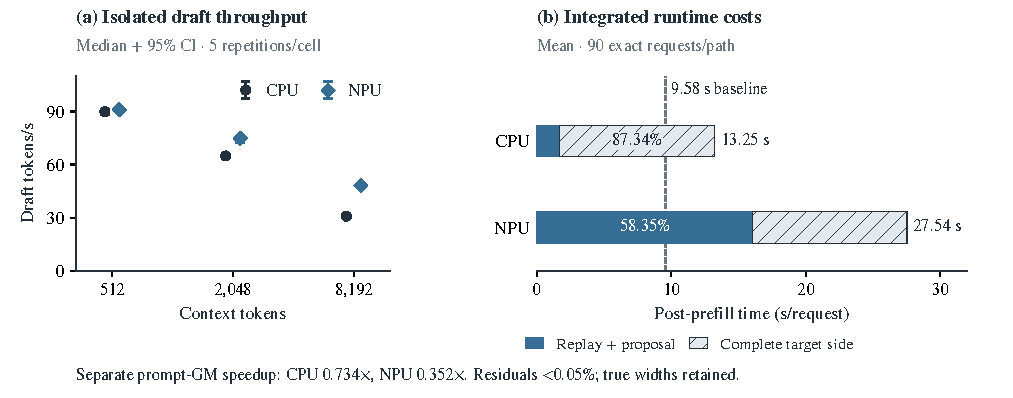
\includegraphics[width=\textwidth]{figures/presentation_v05/pdf/state.pdf}
\caption{\textbf{Isolated draft advantage and complete 358H cost.} A: five-repeat steady-state draft throughput with repetition-bootstrap intervals. B: arithmetic mean post-prefill seconds over 90 exact observations per path, against the shared baseline. NPU's 58.35\% region combines full-prefix replay/reconstruction and proposal; it is inseparable. CPU complete target work is 87.34\%. These bars differ from the prompt-GM speedups in Table~\ref{tab:headlines}; persistence savings are unmeasured.}
\label{fig:state}
\end{figure*}

\subsection{Stateful realization}
\label{sec:state}
On 358H, isolated NPU draft throughput exceeds CPU at tested contexts, but both integrated direct-ID-qualified paths are slower than target-only. Complete committed progress is $C=\HcpuC$ and $\HnpuC$, including correction/bonus. Complete target work consumes \HcpuTarget\% of CPU-path time. The NPU synchronous OpenVINO region combines full-prefix replay/reconstruction and proposal, consuming \HnpuDraft\%; these costs are inseparable. Residual orchestration is \HcpuResidual\% and \HnpuResidual\%.

Figure~\ref{fig:state} describes the measured interface, not NPU capability or a measured persistence benefit. Arithmetic totals give CPU $(\dreal,\rtarget,X)=(\HcpuD,\HcpuR,\HcpuX)$ and NPU $(\HnpuD,\HnpuR,\HnpuX)$, yielding \HcpuAggregate$\times$ and \HnpuAggregate$\times$ in Equation~\ref{eq:normalized}; these are total-time ratios rather than Table~\ref{tab:headlines}'s prompt GMs. With measured progress, target-work and baseline totals fixed, nonnegative draft and residual terms imply $S\le C/\rtarget$: \DerCPUZero$\times$ CPU and \DerNPUZero$\times$ NPU, even if both other terms vanish. Thus draft-only savings cannot reach parity under this accounting. This post-study arithmetic bound is not a prompt-GM bound or an optimization experiment; changing progress or target execution invalidates its fixed assumptions. The later persistent-state/wider-target candidate stops at qualification without formal performance or energy.

\ifruntime\section{Runtime Control under Qualified Fixed Modes}
\label{sec:runtime}
The separate M4 runtime study tests whether continuation control improves a qualified speculative path. It uses its own frozen policy, direct-ID gate and cost boundary; historical M4 timing is background rather than its qualification evidence.

\subsection{A prospective cost guard on M4}
Guard tests a frozen rule against target-only and fixed speculation, using Qwen3-8B/0.6B Q8\_0 on llama.cpp Metal, fixed $k=\RTK$, greedy generation and a \RTCap-token cap. It starts on Always-Spec's path and may fall back permanently to target-only. At eligible completed rounds it divides all charged generation cost by committed progress, including the initial seed and correction/bonus; rejected proposals do not count. It continues when cost per token is at most $(1-m)R_{\mathrm{ref}}$, otherwise falling back after reconciling invalid suffix state. Zero progress also triggers fallback.

Calibration freezes the target reference and selects margin \RTMargin\ with decisions starting after \RTRounds\ rounds. The controller receives no task labels, future length or request-specific oracle. The post-prefill timer charges control and transition costs; Appendix T retains the full rule, grid, tie-breaks and timing boundary.

\subsection{Held-out evaluation}
Historical outcomes informed the design; prospective means policy freeze before reserved outcomes. Exposure exclusion and deterministic selection give disjoint calibration, qualification and held-out splits of \RTCalibration, \RTQualification\ and \RTPrompts\ prompts, balanced across HumanEval and Spec-Bench. Policy and reference precede qualification/formal measurement; the appendix retains the audited freeze-hash metadata defect. Always-Spec and Guard each qualify \RTQualPairs/\RTQualPairs\ direct-ID pairs.

The held-out study runs \RTReps\ repetitions of three conditions on \RTPrompts\ prompts (\RTObservations\ observations), randomizing condition order within prompt/repetition. Both speculative paths preserve \RTExact/\RTExact\ complete direct-ID sequences. Prompt condition medians precede latency ratios and the GM; \RTBootstrap\ prompt-bootstrap draws use seed \RTSeed. The supplement retains exact estimator, exposure and metadata-recovery details.

\begin{table}[t]
\caption{M4 per-prompt median post-prefill latencies. Each speculative condition is \RTExact/\RTExact\ direct-token exact. The offline oracle is unavailable online. The separated Guard/Always-Spec contrast is reviewer-requested post-study paired secondary analysis; values above one mean Guard is slower.}
\label{tab:runtime}
\centering
\begin{tabular}{lcc}
\toprule
Latency ratio & GM & 95\% prompt CI \\
\midrule
\multicolumn{3}{l}{\emph{Speedup versus target-only (higher is faster)}}\\
Target / Guard & \RTGuard & [\RTGuardLo, \RTGuardHi] \\
Target / Always-Spec & \RTAlways & [\RTAlwaysLo, \RTAlwaysHi] \\
\midrule
\multicolumn{3}{l}{\emph{Descriptive hindsight latency ratio}}\\
Guard / offline oracle & \RTOracle & [\RTOracleLo, \RTOracleHi] \\
\midrule
\multicolumn{3}{l}{\emph{Post-study paired secondary latency ratio}}\\
Guard / Always-Spec & \RTSecondary & [\RTSecondaryLo, \RTSecondaryHi] \\
\bottomrule
\end{tabular}
\end{table}

Guard is faster than target-only, but fixed speculation has the higher speedup (Table~\ref{tab:runtime}). A post-study paired comparison gives Guard/Always-Spec latency \RTSecondary\ [\RTSecondaryLo, \RTSecondaryHi], entirely above parity. Guard is faster on \RTGuardFaster\ prompt medians, Always-Spec on \RTAlwaysFaster, with \RTTies\ ties. Fallback occurs in \RTFallback\% of \RTExact\ executions, measuring activity rather than beneficial decisions. Guard/oracle is \RTOracle$\times$; this hindsight oracle chooses the lower target-only or Always-Spec median, not an achievable runtime policy.

Reconstructing all original medians finds target-only faster than Always on only \DerTargetFaster/\RTPrompts\ prompts, both Spec-Bench. Always/oracle is \DerAlwaysOracle$\times$. Choosing the better of these two measured fixed modes after seeing outcomes therefore offers about \DiagMOpportunity\% GM latency reduction from Always, computed from the full-precision ratio. Guard falls back in all six executions of those two prompts but still loses to target-only on their medians. The family-stratified sensitivity analysis also leaves Guard slower (Appendix P). These post-study comparisons estimate neither transition cost nor opportunity for arbitrary within-request switching.

Guard preserves IDs but supplies no incremental benefit over Always-Spec. Fallback activity does not establish beneficial decisions or risk reduction. No runtime energy claim is made. Policy transfer and stable small-stratum effects remain unestablished; the archived policy-freeze defect and original stopped pipeline markers are documented separately.
\fi
\section{System Implications and Research Outlook}
\label{sec:hardwareconclusion}
The prediction studies select reproduction programs; reference gates decide compatibility; cost studies bound optimization opportunity (Table~\ref{tab:decisions}). B570's successful simplification removes draft/proposal dependencies from its frozen reproduction task. RTX's specified capacity-level simplification fails, while proposal-conditioned replay reproduces the complete path. Neither result establishes a minimal state representation or a portable cause.
\begin{table*}[t]
\caption{Engineering uses of the retained results. Reproduction concerns frozen outputs; optimization budgets are conditional and no proposed improvement is measured.}
\label{tab:decisions}
\centering
\begin{tabular}{@{}>{\raggedright\arraybackslash}p{.62in}>{\raggedright\arraybackslash}p{1.58in}>{\raggedright\arraybackslash}p{2.22in}>{\raggedright\arraybackslash}p{1.68in}@{}}
\toprule
Study & Information beyond a basic gate & Reproduction task / optimization decision & Scope of that use \\
\midrule
B570 & Full non-reference suffixes predicted without proposals & Reproduce the tested capped native outputs with target-only UB1; remove draft loading, proposals and native speculative outer loop & Frozen stack and prompts; no measured debugging saving or causal irrelevance \\
RTX A & Candidates with equal totals fail on different tasks; replay succeeds & Reject this UB2 reproducer; retain the sealed tape, locally computed target decisions and KV reconciliation & Shared numerical routines; no minimality or validation of a correction \\
RTX B & Serialization qualifies but loses on every prompt & Exclude measured serialization as a latency optimization & Instrumented post-prefill cost; no qualified batched gain \\
358H & Overhead-only prompt-GM ceilings remain below one & Parity needs a changed premise; even with other cost zero, uniform target-work cuts must reach \DiagCPUReduction\%/\DiagNPUReduction\% & Baseline/progress fixed; necessary optimistic budgets, not achieved savings \\
\ifruntime M4 & About \DiagMOpportunity\% two-fixed-mode opportunity; Guard adds 2.71\% GM latency & Prefer fixed speculation on this aggregate measured workload; assess opportunity before control & Hindsight fixed modes; no bound on arbitrary within-request switching \\
\fi
\bottomrule
\end{tabular}
\end{table*}


\paragraph{Use a tested reproducer for diagnosis.}
On B570, a target-only harness can generate the tested native expected outputs, including non-reference suffixes. On RTX, the successful harness computes its own target decisions while consuming a sealed proposal tape. The complete arrays give expected outputs for regression checks of the frozen paths. Their agreement supplies no evidence that a future correction or changed numerical stack will behave identically; such a use needs agreement back to native execution. The present study demonstrates reproducer selection, not a completed bug fix or measured debugging savings.

\paragraph{Change the cost term that limits the opportunity.}
RTX serialization qualifies but loses within its instrumented boundary. On 358H, removing draft/residual cannot reach parity at fixed target work and progress. Under the optimistic premise that all other cost vanishes, a uniform target-work reduction of at least \DiagCPUReduction\% CPU or \DiagNPUReduction\% NPU is needed for the original prompt-GM ceiling to reach one. A design that changes target execution or committed progress must qualify that new path before claiming a gain. Isolated NPU speed cannot establish it.

\ifruntime
\paragraph{Measure opportunity before adding control.}
Hindsight choice between the two measured fixed modes lowers GM latency from Always by about \DiagMOpportunity\%; Guard instead adds 2.71\%. This small fixed-mode opportunity helps explain why fallback activity alone is weak evidence of useful control. It does not bound policies that change the execution or switch within a request.
\else
The full manuscript separately assesses M4 control and its limited opportunity between two measured fixed modes.
\fi

A useful next diagnostic study would test whether a simpler reproducer helps isolate a discrepancy or validate a correction, then confirm the result on native execution. Stronger causal attribution instead needs a discriminating state/trace-matched contrast and controlled continuation. These are additional research questions; full-array agreement alone cannot answer them. The conclusions here remain the tested reproduction choices and conditional cost budgets.

\section{Related Work}
\label{sec:related}
\paragraph{Performance and heterogeneous execution.}
Speculative decoding amortizes target computation under its algorithmic assumptions \citep{leviathan2023}. Prior work already documents verification and workload limits: \citet{illusion} study verification dominance and batch effects in vLLM; \citet{specllm} account for conditional execution cost and runtime control; \citet{distance} derive edge--cloud profitability conditions. On consumer Apple silicon, \citet{lossless} reports gains and slowdowns across five backend configurations, diagnoses ineffective batch-parallel verification in one quantized Metal path, tests output agreement, and observes target-only batch-shape argmax changes. Slowdown and correctness gating have already been studied, as has heterogeneous placement: Dovetail, DuoDecoding, and Mirror-SD study GPU/CPU or GPU/NPU paths \citep{dovetail,duodecoding,mirror}; \citet{compilerassisted} combine an analytical cost model with compiler-oriented CPU/GPU partitioning, and Lever jointly optimizes draft, verification, and CPU/NPU execution for a smartphone target \citep{lever}. State reuse has prior art in compressed draft KV memory \citep{compactmemory}. Our 358H study measures one interface that combines replay and proposal; it establishes no general placement or persistence result.

\paragraph{Numerical paths and output contracts.}
The separate appendix compares the closest prior questions. Numerical sensitivity, deterministic inference construction, correctness forensics and cost gating are established prior work. LLM-42 uses fixed-shape verification and KV repair to construct deterministic inference \citep{llm42}; our tests forecast finite native paths and do not establish that guarantee. Our controlled studies retain complete output forecasts and paired reference effects, but the new RTX bridge also establishes a strong ordinary target-only alternative. We therefore make no general prediction-method or efficiency claim. MarginGate gates deterministic verification by a calibrated logit margin and repairs the current KV column \citep{margingate}; our post-outcome score observations supply neither that policy nor a competing repair guarantee. Fixed-prefix precision controls and bidirectional cache transplantation show how replay divergence can follow live KV state \citep{stagereplay}. Our shared prefixes do not supply such a causal transplantation test. Integer Alibi localizes cross-kernel differences under verified shared-operand, nonoverflowing INT8 accumulation assumptions \citep{integeralibi}; those assumptions are not established for our Q8\_0 runtime dispatch. We identify no unique arithmetic operation.
\citet{vosti} formalize and verify fixed-deployment determinism through engine invariants and relational kernel contracts, including prefill/decode and KV-cache changes. Their bitwise-logit specification is stronger than our finite generated-ID comparisons. We forecast tested paths that can remain reference-incompatible; we supply neither an engine proof nor a deterministic implementation guarantee.


\paragraph{Adaptive speculation and the study boundary.}
TurboSpec adjusts speculation for serving goodput \citep{turbospec}; BanditSpec selects configurations online \citep{banditspec}; ACL HeteroSpec adapts verification from contextual entropy \citep{aclheterospec}. Adaptive control is established prior work. Our M4 Guard is a qualified runtime control test, not a new policy advantage: it beats target-only, but fixed speculation is faster in the post-study paired secondary comparison. Our measurements test prospective direct-ID qualification, frozen trajectory prediction, sampled intervention effects and realized cost on qualified paths.

\section{Limitations}
\label{sec:limitations}
This study covers four consumer systems and a narrow Qwen3 model family. Hardware, operating systems, runtime versions, backends, and some quantization choices co-vary. The observed failures of local indicators are case evidence, not an estimated population-wide failure rate or a controlled portability benchmark. The diagnosed mechanisms are not exhaustive and do not causally explain the M4 workload contrast. The results establish observed regimes and within-platform mechanisms, not an architectural ranking or a general deployment law. Serving concurrency, production load, and broader model families are outside the measured scope.

Token equivalence is deliberately strict and conditional on the frozen reference; a different quality contract could admit other paths. HumanEval functional execution and pass@$k$ were not evaluated. Serialized B570 outputs still mismatch, and the CUDA evidence is bounded to the captured stack and case. No claim of general backend unsuitability follows.

Campaign-specific estimators and bootstrap implementations differ. Prompt intervals do not cover all system-state uncertainty, including M4 session/thermal effects. The M4 corrected synthetic-ceiling preregistration remains unexecuted. Decode timing excludes initial prefill and loading, so it is not whole-request user latency. Energy sensor domains differ; there is no global energy ranking or end-to-end 358H Phase-3 energy claim.

Windows raw per-run provenance is weaker than that of the other closed campaigns. The 358H draft-source reconstruction is \texttt{STRONGLY\_SUPPORTED}, not proven historical upstream identity. Replay and proposal are measured together, preventing separate causal timing attribution to either. No measured runtime intervention exists in this version; persistent state, path selection, and profitability control remain proposals. These limitations bound the hardware conclusion independently of the future software decision.

\section{Conclusion}
\label{sec:conclusion}
Fresh direct-ID studies qualify RTX serialization but leave B570 blocked, without a matched fresh latency endpoint. On the tested B570 stack, a frozen target-only UB1 predictor matches 72/72 capped generated-ID runs across 24 repeat-stable prompts; four prompts (12 runs) diverge from the reference. This is predictive sufficiency on that path, not a unique cause or controlled live-loop intervention. On 358H, the combined replay/reconstruction-plus-proposal interface consumes an isolated draft-device advantage; its later intervention stops at qualification. M4 Guard preserves direct-ID output and beats target-only (\RTGuard$\times$), but fixed speculation (\RTAlways$\times$) wins the post-study paired comparison; no incremental control benefit is shown.

\label{maintextend}
\clearpage
\bibliographystyle{mlsys2025}
\bibliography{references}
\end{document}
